%%%%%%%%%%%%%%%%%%%%%%%%%%%%%%%%%%%%%%%%%%%%%%%%%%%%%%%%%%%%%%%%%%%%%%
% LaTeX Example: Project Report
%
% Source: http://www.howtotex.com
%
% Feel free to distribute this example, but please keep the referral
% to howtotex.com
% Date: March 2011 
% 
%%%%%%%%%%%%%%%%%%%%%%%%%%%%%%%%%%%%%%%%%%%%%%%%%%%%%%%%%%%%%%%%%%%%%%
% How to use writeLaTeX: 
%
% You edit the source code here on the left, and the preview on the
% right shows you the result within a few seconds.
%
% Bookmark this page and share the URL with your co-authors. They can
% edit at the same time!
%
% You can upload figures, bibliographies, custom classes and
% styles using the files menu.
%
% If you're new to LaTeX, the wikibook is a great place to start:
% http://en.wikibooks.org/wiki/LaTeX
%
%%%%%%%%%%%%%%%%%%%%%%%%%%%%%%%%%%%%%%%%%%%%%%%%%%%%%%%%%%%%%%%%%%%%%%
% Edit the title below to update the display in My Documents
%\title{Project Report}
%
%%% Preamble
\documentclass[paper=a4, fontsize=11pt]{scrartcl}
\usepackage[T1]{fontenc}
\usepackage{fourier}
\usepackage{listings}
\usepackage[english]{babel}															% English language/hyphenation
\usepackage[protrusion=true,expansion=true]{microtype}	
\usepackage{amsmath,amsfonts,amsthm} % Math packages
\usepackage[pdftex]{graphicx}	
\usepackage{url}


%%% Custom sectioning
\usepackage{sectsty}
\allsectionsfont{\centering \normalfont\scshape}


%%% Custom headers/footers (fancyhdr package)
\usepackage{fancyhdr}
\pagestyle{fancyplain}
\fancyhead{}											% No page header
\fancyfoot[L]{}											% Empty 
\fancyfoot[C]{}											% Empty
\fancyfoot[R]{\thepage}									% Pagenumbering
\renewcommand{\headrulewidth}{0pt}			% Remove header underlines
\renewcommand{\footrulewidth}{0pt}				% Remove footer underlines
\setlength{\headheight}{13.6pt}


%%% Equation and float numbering
\numberwithin{equation}{section}		% Equationnumbering: section.eq#
\numberwithin{figure}{section}			% Figurenumbering: section.fig#
\numberwithin{table}{section}				% Tablenumbering: section.tab#


%%% Maketitle metadata
\newcommand{\horrule}[1]{\rule{\linewidth}{#1}} 	% Horizontal rule

\title{
		%\vspace{-1in} 	
		\usefont{OT1}{bch}{b}{n}
		\normalfont \normalsize \textsc{University of Illinois at Urbana-Champaign} \\ [25pt]
		\horrule{0.5pt} \\[0.4cm]
		\huge Assignment 2 - Report \\
		\horrule{2pt} \\[0.5cm]
}
\author{
		\normalfont 								\normalsize
        Zhenye Na (zna2)\\[-3pt]		\normalsize
        \today
}
\date{}


%%% Begin document
\begin{document}
\maketitle

\section{Short Questions}
Provide a short answer (3-4 sentences at most) for each of the following questions. You may use figures if necessary.

\begin{enumerate}
	\item Suppose we have a relation R as given below, representing the exam statistics for course CS411. First project relation R to GPA (i.e., eliminate SID and Name) and then calculate the average GPA, under the set-model and the bag-model respectively. Which model is preferred in this example and why?\\
	\centerline{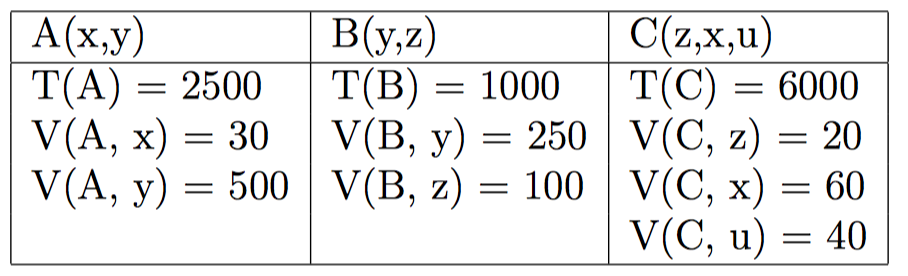
\includegraphics[scale=0.5]{1.jpg}}\\
    \textbf{Answer:} We should use Bag Operations. It is faster than sets because of no duplicate elimination in Bag Operations.
    
	\item Consider a relation \textit{R(A, B, C)}. You may assume there are no null values or duplicates in R. If the result of 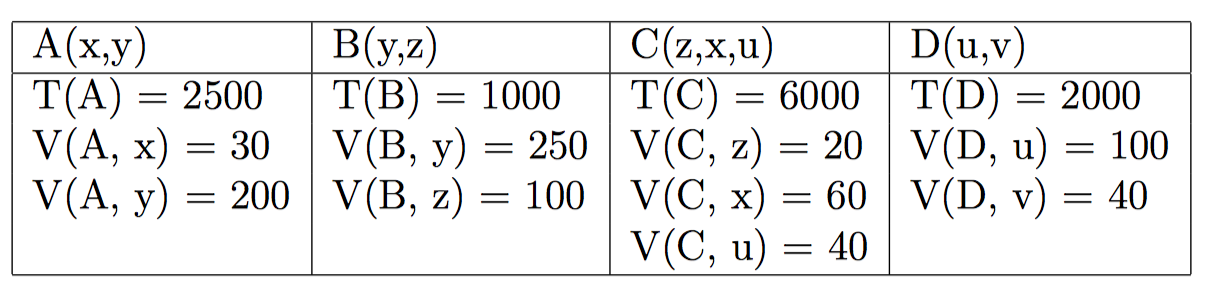
\includegraphics[height=\baselineskip]{2.jpg} is always guaranteed to be empty, then what property of R can you infer? (Hint: think functional dependencies.)\\
	\textbf{Answer:} There exists a FD: $A \rightarrow B$ in relation \textit{R}.
    
	\item Consider any relation R that never contains more than one tuple. Is it true that R must in Boyce-Codd Normal Form (BCNF)? Justify your answer.\\
    \textbf{Answer:} \textbf{True}. Whether relation R is a BCNF is determined by whether LHS is super-key (closure) of the relation. However, here we have only one instance so it will always be BCNF.
    
	\item Consider a relation \textit{R(A, B, C, D, E)} with dependencies \textit{AB} $\rightarrow$ \textit{CD}, \textit{C} $\rightarrow$ \textit{AB}, \textit{D} $\rightarrow$ \textit{AE}, list all minimal keys for R. Also, state whether the relation R is in 3NF \textbf{with reasoning}.\\
    \textbf{Answer:} Minimal keys for R are \big\{A, B\big\}, \big\{C\big\}, \big\{D, B\big\}.\\
    It is not a 3NF.\\
    Minimal Basis: \big\{ABC\big\}, \big\{ABD\big\}, \big\{AC\big\}, \big\{BC\big\}, \big\{AD\big\}, \big\{DE\big\}. This is the 3NF decomposition for this relation.
    
    \item Two sets of functional dependencies (FD's) \textit{F} and \textit{F}' are equivalent if all FD's in \textit{F}' follow from the ones in \textit{F}, and all FD's in \textit{F} follow from the ones in \textit{F}' . Consider the following three sets of functional dependencies:\\
    
      \begin{itemize}
        \item \textit{F1 = A $\rightarrow$ C, B $\rightarrow$ A}
        \item \textit{F2 = B $\rightarrow$ AC}
        \item \textit{F3 = AB $\rightarrow$ C, B $\rightarrow$ A}
      \end{itemize}
    
    \begin{enumerate}
    \item Are \textit{F}1 and \textit{F}2 equivalent? Justify your answer.\\
    \textbf{Answer:} False. Use transitivity in \textit{F1} we can get $B \rightarrow A, B \rightarrow C$. However, we cannot get $ A \rightarrow C$ from \textit{F}2.
    
    \item Are \textit{F}1 and \textit{F}3 equivalent? Justify your answer.\\
    \textbf{Answer:} False. Use transitivity in \textit{F1} we can get $B \rightarrow A, B \rightarrow C$. In \textit{F}3, $B \rightarrow A \Rightarrow B \rightarrow AB \Rightarrow B \rightarrow C$. However, we cannot get $ A \rightarrow C$ from \textit{F}3.
    
    \item Are \textit{F}2 and \textit{F}3 equivalent? Justify your answer.\\
    \textbf{Answer:} True. In \textit{F}3, $B \rightarrow A \Rightarrow B \rightarrow AB \Rightarrow B \rightarrow C$. In \textit{F}2, $B \rightarrow AC$. They are equivalent.
    
    \end{enumerate}

\end{enumerate}


\section{Relational algebra to English}
Consider a relation Works (\underline{name}, company, salary) with no duplicates. Consider the following
relational algebra expression, written in linear notation.

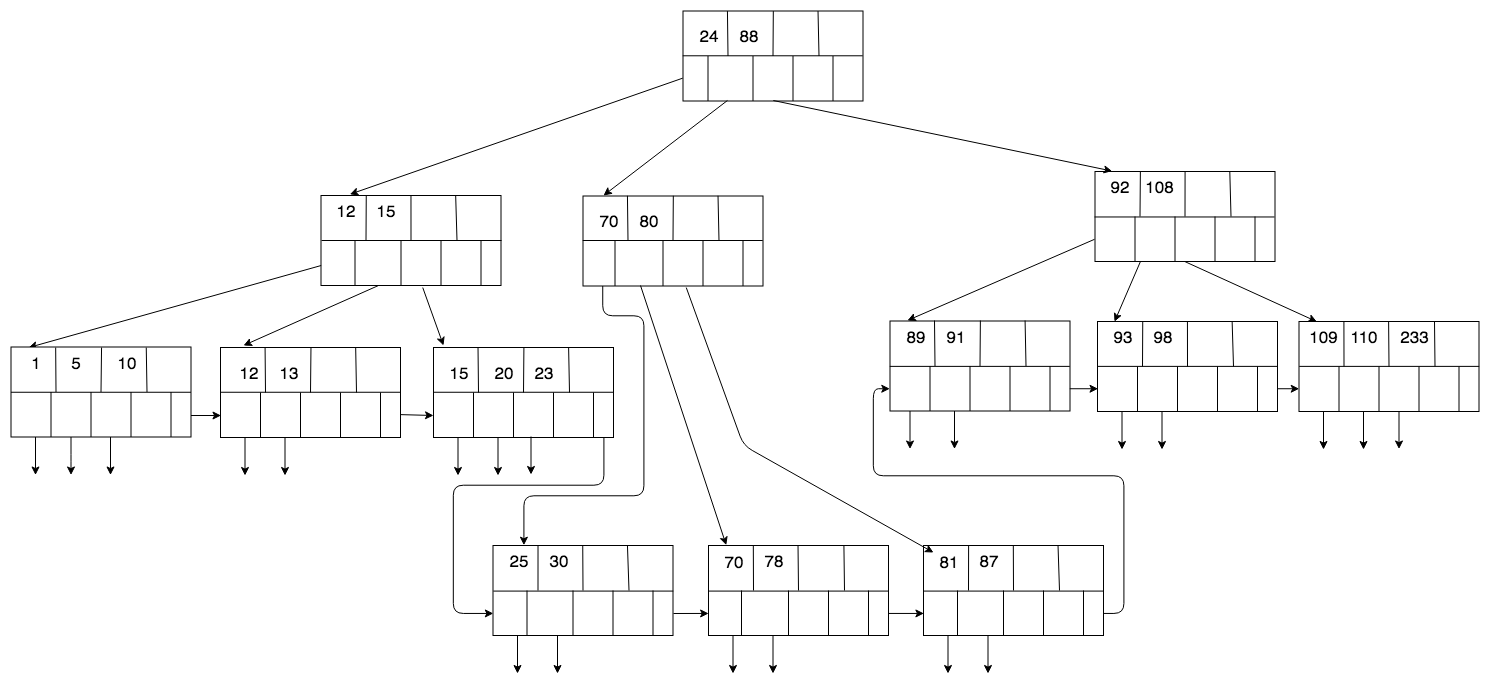
\includegraphics[scale=0.5]{4.jpg}

State in English what is computed as the final answer briefly. Long-winded answers will
be deducted points. For partial credit, explain what \textit{P}1, \textit{P}2 and \textit{P}3 contain.\\
\textbf{Answer: }
\textit{Answer(name)}: Select people's name, who have salary higher than the highest salary in IBM.


\section{English to Relational Algebra}
Consider the following relational database schema that describes information about students
and their courses. A course is uniquely identified by its CODE (e.g., "CS411"), and a student
is uniquely identified by his or her SID.\\
Course(\underline{CODE}, units, time, room) // all courses\\
Student(\underline{SID}, name, level) // all students, level can be "grad" or "undergrad"\\
Taking(\underline{SID}, \underline{CODE}) // current enrollment information\\

Write a relational algebra expression to list the information (i.e., CODE, units, time, room) of courses that are currently offered but have no graduate students enrolled.

\begin{displaymath} 
Course \leftarrow \Big(\Pi_{(code)} \big(\sigma_{(level \neq 'grad')}(Student \bowtie Course)\big)\Big) \bowtie Course
\end{displaymath}

\section{Data to functional dependency}
Consider a relation R(A, B, C), satisfying some functional dependency. Two instances of R are given as below:

	\centerline{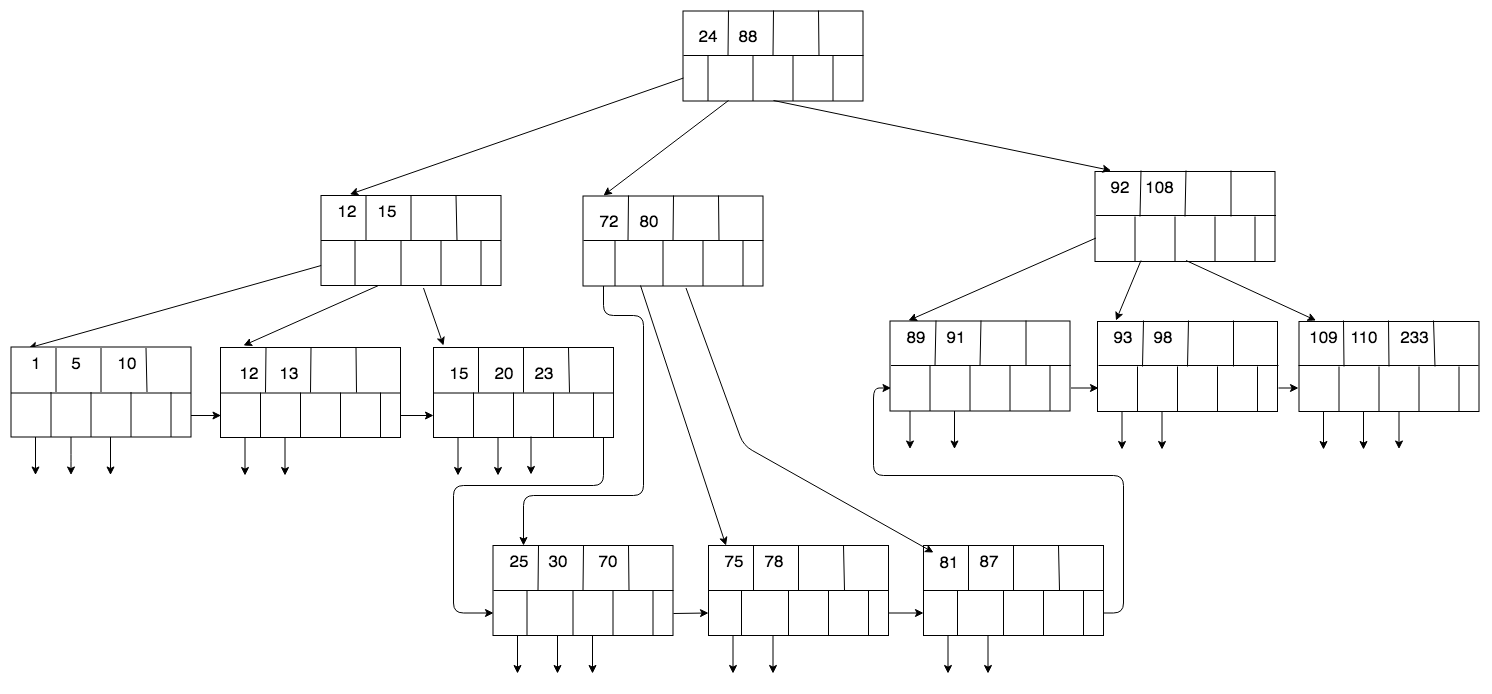
\includegraphics[scale=0.5]{3.jpg}}

Based on R's schema, enumerate all possible completely nontrivial functional dependencies (FDs) with only a single attribute on the right-hand side. Then, based on the instances above, for each FD you listed, label whether it:\\
H: Definitely holds in R.\\
NH: Definitely does not hold in R.\\
CD: Cannot be determined from the information given whether or not it holds in R.
\begin{itemize}
\item $\textit{B} \rightarrow \textit{A}$: NH in R.
\item $\textit{C} \rightarrow \textit{A}$: NH in R.
\item $\textit{BC} \rightarrow \textit{A}$: NH in R.

\item $\textit{A} \rightarrow \textit{B}$: NH in R.
\item $\textit{C} \rightarrow \textit{B}$: CD in R.
\item $\textit{AC} \rightarrow \textit{B}$: CD in R.

\item $\textit{A} \rightarrow \textit{C}$: NH in R.
\item $\textit{B} \rightarrow \textit{C}$: CD in R.
\item $\textit{AB} \rightarrow \textit{C}$: CD in R.
\end{itemize}


\section{Normalization}
Consider the following relational schema for a chain store:\\
Sale(clerk, store, city, date, dish, size)\\
// a clerk sold a dish on a particular day at a given store in a city\\
Menu(dish, size, price)\\
// prices and available size for the dish\\

Make the following assumptions:
\begin{itemize}
\item Each clerk works in one store.
\item Each store is in one city.
\item The price of a dish is different for different sizes. The store has standardized prices:
the same sized dish cannot be sold to two persons at two different prices.
\end{itemize}


\begin{enumerate}
\item Specify a set of completely nontrivial functional dependencies for relations Sale and Menu that encodes the assumptions described above and no additional assumptions.
$clerk \rightarrow store$\\
$store \rightarrow city$\\
$dish, size \rightarrow price$\\

\item Based on your functional dependencies in part (1), specify all minimal keys for relations Sale and Menu.\\
\textbf{Sale: } \{clerk, date, dish, size\}\\
\textbf{Menu: } \{dish, size\}

\item Are the schema of Sale and Menu in Boyce-Codd Normal Form (BCNF) according to
your answers to (1) and (2)? If not, give a decomposition into BCNF. If yes, justify your answer.\\
For Menu, it is in Boyce-Codd Normal Form (BCNF). However, Sale is not in BCNF.\\
\textbf{Menu: } The closure for the minimal key in previous question is \{dish, size, price\}. It contains all the attributes in Menu schema.\\
\textbf{Sale: }\\
- \{clerk, store\}\\
- \{store, city\}\\
- \{clerk, date, dish, size\}

\item Now add the following assumption:

\begin{itemize}
\item Each city has at most one store and each store has only one clerk.
\end{itemize}
Specify additional functional dependencies to take these new assumptions into account.\\
\textbf{Answer: }$city \rightarrow store,\;store \rightarrow clerk$

\item Based on your functional dependencies for parts (1) and (4) together, specify all minimal keys for relation Sale.\\
\textbf{Sale: }\\
- \{clerk, date, dish, size \}\\
- \{store, date, dish, size \}\\
- \{city, date, dish, size \}\\

\item Are the schema of Sale and Menu in 3NF according to your answers to (1), (4) and (5)? If not, give a decomposition into 3NF. If yes, justify your answer.\\
\textbf{Answer: }Sale is not 3NF, Menu is 3NF.\\
\textbf{Sale: }(clerk, store), (store, city), (clerk, date, dish, size)\\
\textbf{Menu: }$dish, size \rightarrow price$, so (dish, size, price) is the minimal-key, the result from step 2. We do not need decompose this.

\end{enumerate}




%%% End document
\end{document}